\documentclass[twoside]{book}

% Packages required by doxygen
\usepackage{calc}
\usepackage{doxygen}
\usepackage{graphicx}
\usepackage[utf8]{inputenc}
\usepackage{makeidx}
\usepackage{multicol}
\usepackage{multirow}
\usepackage{textcomp}
\usepackage[table]{xcolor}

% Font selection
\usepackage[T1]{fontenc}
\usepackage{mathptmx}
\usepackage[scaled=.90]{helvet}
\usepackage{courier}
\usepackage{amssymb}
\usepackage{sectsty}
\renewcommand{\familydefault}{\sfdefault}
\allsectionsfont{%
  \fontseries{bc}\selectfont%
  \color{darkgray}%
}
\renewcommand{\DoxyLabelFont}{%
  \fontseries{bc}\selectfont%
  \color{darkgray}%
}

% Page & text layout
\usepackage{geometry}
\geometry{%
  a4paper,%
  top=2.5cm,%
  bottom=2.5cm,%
  left=2.5cm,%
  right=2.5cm%
}
\tolerance=750
\hfuzz=15pt
\hbadness=750
\setlength{\emergencystretch}{15pt}
\setlength{\parindent}{0cm}
\setlength{\parskip}{0.2cm}
\makeatletter
\renewcommand{\paragraph}{%
  \@startsection{paragraph}{4}{0ex}{-1.0ex}{1.0ex}{%
    \normalfont\normalsize\bfseries\SS@parafont%
  }%
}
\renewcommand{\subparagraph}{%
  \@startsection{subparagraph}{5}{0ex}{-1.0ex}{1.0ex}{%
    \normalfont\normalsize\bfseries\SS@subparafont%
  }%
}
\makeatother

% Headers & footers
\usepackage{fancyhdr}
\pagestyle{fancyplain}
\fancyhead[LE]{\fancyplain{}{\bfseries\thepage}}
\fancyhead[CE]{\fancyplain{}{}}
\fancyhead[RE]{\fancyplain{}{\bfseries\leftmark}}
\fancyhead[LO]{\fancyplain{}{\bfseries\rightmark}}
\fancyhead[CO]{\fancyplain{}{}}
\fancyhead[RO]{\fancyplain{}{\bfseries\thepage}}
\fancyfoot[LE]{\fancyplain{}{}}
\fancyfoot[CE]{\fancyplain{}{}}
\fancyfoot[RE]{\fancyplain{}{\bfseries\scriptsize Generated on Sun Nov 2 2014 18\-:16\-:53 for G\-U\-I by Doxygen }}
\fancyfoot[LO]{\fancyplain{}{\bfseries\scriptsize Generated on Sun Nov 2 2014 18\-:16\-:53 for G\-U\-I by Doxygen }}
\fancyfoot[CO]{\fancyplain{}{}}
\fancyfoot[RO]{\fancyplain{}{}}
\renewcommand{\footrulewidth}{0.4pt}
\renewcommand{\chaptermark}[1]{%
  \markboth{#1}{}%
}
\renewcommand{\sectionmark}[1]{%
  \markright{\thesection\ #1}%
}

% Indices & bibliography
\usepackage{natbib}
\usepackage[titles]{tocloft}
\setcounter{tocdepth}{3}
\setcounter{secnumdepth}{5}
\makeindex

% Hyperlinks (required, but should be loaded last)
\usepackage{ifpdf}
\ifpdf
  \usepackage[pdftex,pagebackref=true]{hyperref}
\else
  \usepackage[ps2pdf,pagebackref=true]{hyperref}
\fi
\hypersetup{%
  colorlinks=true,%
  linkcolor=blue,%
  citecolor=blue,%
  unicode%
}

% Custom commands
\newcommand{\clearemptydoublepage}{%
  \newpage{\pagestyle{empty}\cleardoublepage}%
}


%===== C O N T E N T S =====

\begin{document}

% Titlepage & ToC
\hypersetup{pageanchor=false}
\pagenumbering{roman}
\begin{titlepage}
\vspace*{7cm}
\begin{center}%
{\Large G\-U\-I }\\
\vspace*{1cm}
{\large Generated by Doxygen 1.8.6}\\
\vspace*{0.5cm}
{\small Sun Nov 2 2014 18:16:53}\\
\end{center}
\end{titlepage}
\clearemptydoublepage
\tableofcontents
\clearemptydoublepage
\pagenumbering{arabic}
\hypersetup{pageanchor=true}

%--- Begin generated contents ---
\chapter{Hierarchical Index}
\section{Class Hierarchy}
This inheritance list is sorted roughly, but not completely, alphabetically\-:\begin{DoxyCompactList}
\item Q\-Udp\-Socket\begin{DoxyCompactList}
\item \contentsline{section}{Udp\-Socket}{\pageref{classUdpSocket}}{}
\end{DoxyCompactList}
\item Q\-Widget\begin{DoxyCompactList}
\item \contentsline{section}{Window}{\pageref{classWindow}}{}
\end{DoxyCompactList}
\item Qwt\-Plot\begin{DoxyCompactList}
\item \contentsline{section}{Plot}{\pageref{classPlot}}{}
\end{DoxyCompactList}
\end{DoxyCompactList}

\chapter{Class Index}
\section{Class List}
Here are the classes, structs, unions and interfaces with brief descriptions\-:\begin{DoxyCompactList}
\item\contentsline{section}{\hyperlink{classPlot}{Plot} \\*2\-D display widget }{\pageref{classPlot}}{}
\item\contentsline{section}{\hyperlink{classUdpSocket}{Udp\-Socket} \\*Socket udp of the remote pc }{\pageref{classUdpSocket}}{}
\item\contentsline{section}{\hyperlink{classWindow}{Window} \\*Main window of the G\-U\-I }{\pageref{classWindow}}{}
\end{DoxyCompactList}

\chapter{Class Documentation}
\hypertarget{classPlot}{\section{Plot Class Reference}
\label{classPlot}\index{Plot@{Plot}}
}


2\-D display widget  




{\ttfamily \#include $<$Plot.\-h$>$}

Inheritance diagram for Plot\-:\begin{figure}[H]
\begin{center}
\leavevmode
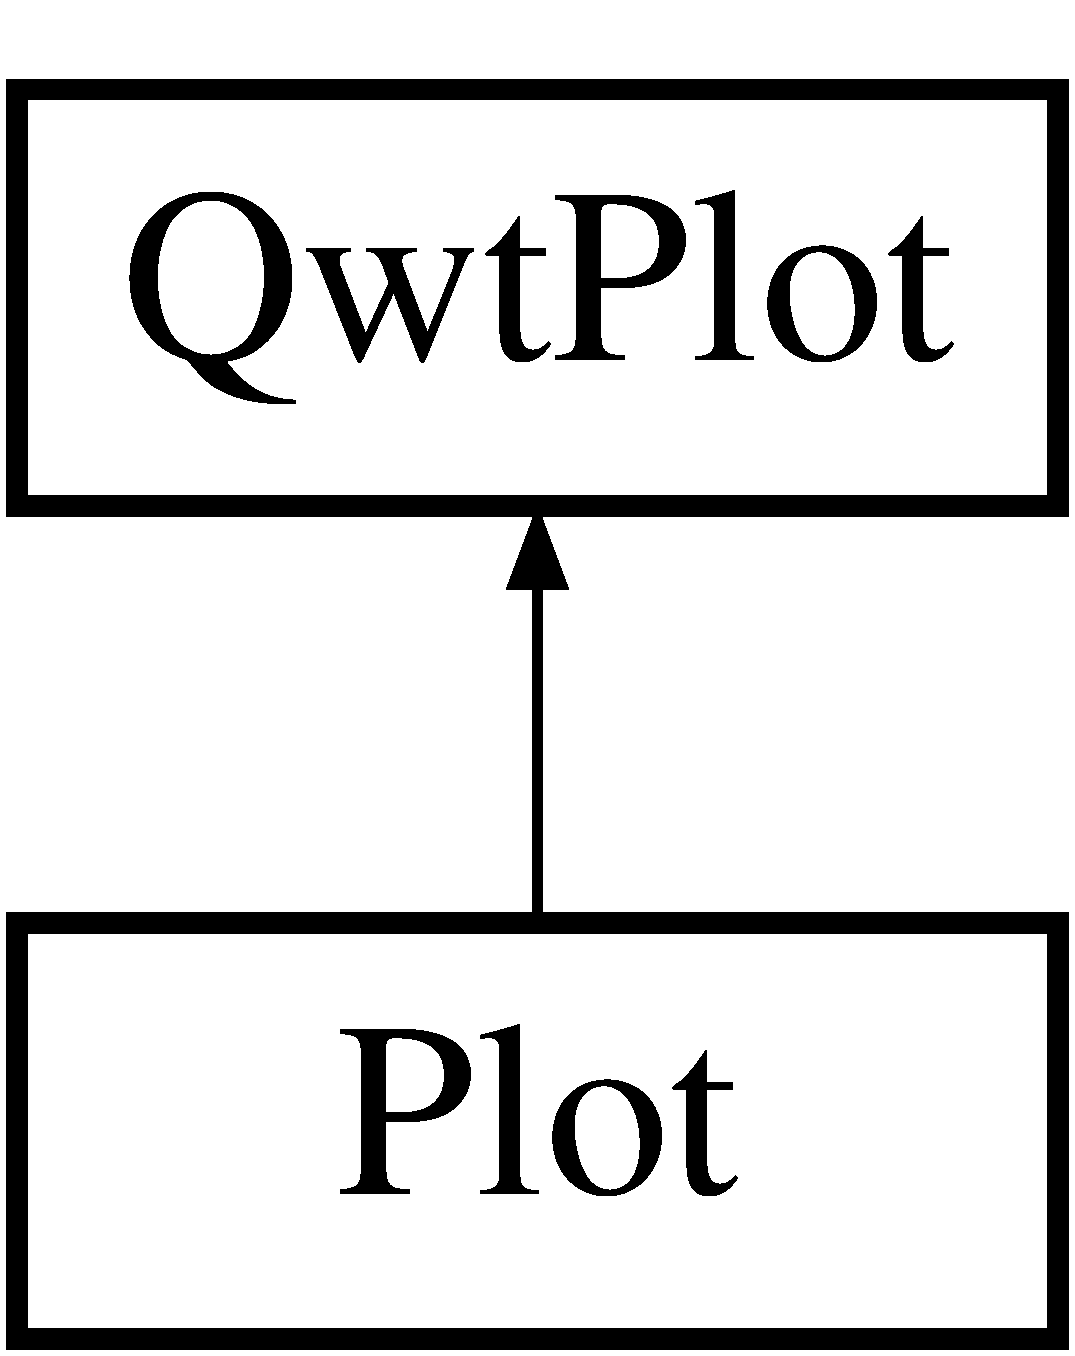
\includegraphics[height=2.000000cm]{classPlot}
\end{center}
\end{figure}
\subsection*{Public Member Functions}
\begin{DoxyCompactItemize}
\item 
\hypertarget{classPlot_a5eace135e8f9b8c0bd89e2b0e24f1387}{{\bfseries Plot} (Q\-Widget $\ast$parent)}\label{classPlot_a5eace135e8f9b8c0bd89e2b0e24f1387}

\item 
\hypertarget{classPlot_a3bc3ac75ac24d391b15df0a5f1f9b4e4}{virtual void {\bfseries draw\-Canvas} (Q\-Painter $\ast$painter)}\label{classPlot_a3bc3ac75ac24d391b15df0a5f1f9b4e4}

\item 
\hypertarget{classPlot_af2a97dc7b52d3adfd23b199e1c318caf}{void {\bfseries set\-Pos\-X} (int x)}\label{classPlot_af2a97dc7b52d3adfd23b199e1c318caf}

\item 
\hypertarget{classPlot_ad85fa5495b49b1bdda900df70bc20183}{void {\bfseries set\-Pos\-Y} (int y)}\label{classPlot_ad85fa5495b49b1bdda900df70bc20183}

\end{DoxyCompactItemize}


\subsection{Detailed Description}
2\-D display widget 

This class inherits Qwt\-Plot and allow to display a two dimensionel graph. \par
It is used for a 2\-D display of the drone's position. 

The documentation for this class was generated from the following files\-:\begin{DoxyCompactItemize}
\item 
/home/mathieu/drone-\/project/pc-\/linux/src/Plot.\-h\item 
/home/mathieu/drone-\/project/pc-\/linux/src/Plot.\-cpp\end{DoxyCompactItemize}

\hypertarget{classUdpSocket}{\section{Udp\-Socket Class Reference}
\label{classUdpSocket}\index{Udp\-Socket@{Udp\-Socket}}
}


Socket udp of the remote pc.  




{\ttfamily \#include $<$Udp\-Socket.\-h$>$}

Inheritance diagram for Udp\-Socket\-:\begin{figure}[H]
\begin{center}
\leavevmode
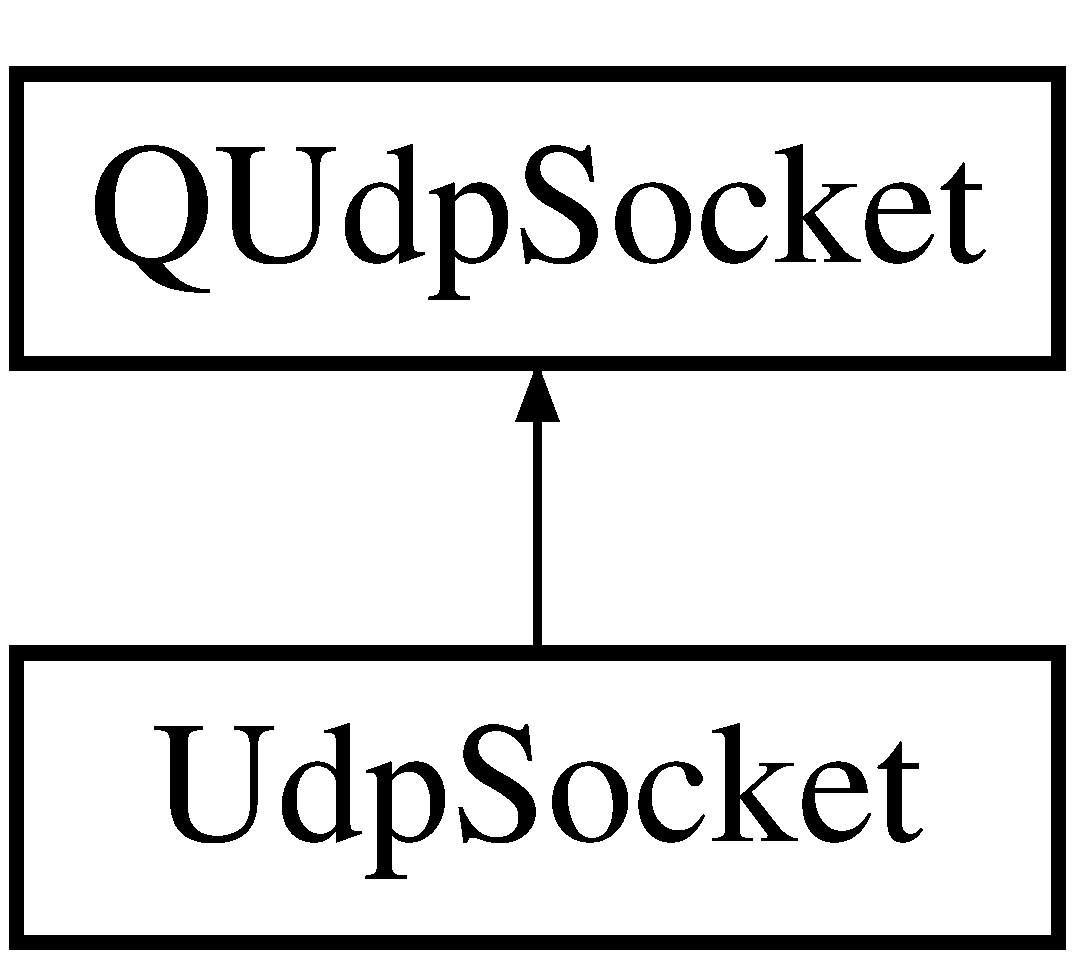
\includegraphics[height=2.000000cm]{classUdpSocket}
\end{center}
\end{figure}
\subsection*{Public Slots}
\begin{DoxyCompactItemize}
\item 
void \hyperlink{classUdpSocket_a3aba1f82aae7c3dc2b0b8487740a4c46}{write} ()
\begin{DoxyCompactList}\small\item\em Send a wifi\-Frame to the drone. \end{DoxyCompactList}\item 
void \hyperlink{classUdpSocket_a4f575273cf1629ed4a46d33b9d955100}{read} ()
\begin{DoxyCompactList}\small\item\em Read the wifi\-Frame received from the drone. \end{DoxyCompactList}\end{DoxyCompactItemize}
\subsection*{Public Member Functions}
\begin{DoxyCompactItemize}
\item 
\hyperlink{classUdpSocket_acd386cff2c60fcd786883c8cfa117df8}{Udp\-Socket} ()
\begin{DoxyCompactList}\small\item\em Constructor. \end{DoxyCompactList}\item 
void \hyperlink{classUdpSocket_abab90176dae0818d9025f605209e0ce3}{process\-Datagram} (wifi\-Frame wf)
\begin{DoxyCompactList}\small\item\em Extract the data from the frame. \end{DoxyCompactList}\item 
\hypertarget{classUdpSocket_ad9113c74edc6e658057f5d6e42311d37}{int {\bfseries get\-Pos\-X} ()}\label{classUdpSocket_ad9113c74edc6e658057f5d6e42311d37}

\item 
\hypertarget{classUdpSocket_a07cf9a3e1a2d5cb67d78a27acd705538}{int {\bfseries get\-Pos\-Y} ()}\label{classUdpSocket_a07cf9a3e1a2d5cb67d78a27acd705538}

\item 
\hypertarget{classUdpSocket_ac99a86841514a4ef770763ff182b20e1}{int {\bfseries get\-Pos\-Z} ()}\label{classUdpSocket_ac99a86841514a4ef770763ff182b20e1}

\end{DoxyCompactItemize}


\subsection{Detailed Description}
Socket udp of the remote pc. 

This class allows to read frames or to send them to the drone \par
Getters allow the user interface to get the positions received and update their displays 

\subsection{Constructor \& Destructor Documentation}
\hypertarget{classUdpSocket_acd386cff2c60fcd786883c8cfa117df8}{\index{Udp\-Socket@{Udp\-Socket}!Udp\-Socket@{Udp\-Socket}}
\index{Udp\-Socket@{Udp\-Socket}!UdpSocket@{Udp\-Socket}}
\subsubsection[{Udp\-Socket}]{\setlength{\rightskip}{0pt plus 5cm}Udp\-Socket\-::\-Udp\-Socket (
\begin{DoxyParamCaption}
{}
\end{DoxyParamCaption}
)}}\label{classUdpSocket_acd386cff2c60fcd786883c8cfa117df8}


Constructor. 

Bind a port in share\-Adress mode. 

\subsection{Member Function Documentation}
\hypertarget{classUdpSocket_abab90176dae0818d9025f605209e0ce3}{\index{Udp\-Socket@{Udp\-Socket}!process\-Datagram@{process\-Datagram}}
\index{process\-Datagram@{process\-Datagram}!UdpSocket@{Udp\-Socket}}
\subsubsection[{process\-Datagram}]{\setlength{\rightskip}{0pt plus 5cm}void Udp\-Socket\-::process\-Datagram (
\begin{DoxyParamCaption}
\item[{wifi\-Frame}]{wf}
\end{DoxyParamCaption}
)}}\label{classUdpSocket_abab90176dae0818d9025f605209e0ce3}


Extract the data from the frame. 

Update the positions atributes of the class with the data received \hypertarget{classUdpSocket_a4f575273cf1629ed4a46d33b9d955100}{\index{Udp\-Socket@{Udp\-Socket}!read@{read}}
\index{read@{read}!UdpSocket@{Udp\-Socket}}
\subsubsection[{read}]{\setlength{\rightskip}{0pt plus 5cm}void Udp\-Socket\-::read (
\begin{DoxyParamCaption}
{}
\end{DoxyParamCaption}
)\hspace{0.3cm}{\ttfamily [slot]}}}\label{classUdpSocket_a4f575273cf1629ed4a46d33b9d955100}


Read the wifi\-Frame received from the drone. 

It emits a signal to update the user interface with the values received. If the wifi frame is a discovery frame, it sends back the frame to the drone. \hypertarget{classUdpSocket_a3aba1f82aae7c3dc2b0b8487740a4c46}{\index{Udp\-Socket@{Udp\-Socket}!write@{write}}
\index{write@{write}!UdpSocket@{Udp\-Socket}}
\subsubsection[{write}]{\setlength{\rightskip}{0pt plus 5cm}void Udp\-Socket\-::write (
\begin{DoxyParamCaption}
{}
\end{DoxyParamCaption}
)\hspace{0.3cm}{\ttfamily [slot]}}}\label{classUdpSocket_a3aba1f82aae7c3dc2b0b8487740a4c46}


Send a wifi\-Frame to the drone. 

Also used in local to test the behaviour in reception 

The documentation for this class was generated from the following files\-:\begin{DoxyCompactItemize}
\item 
/home/mathieu/drone-\/project/pc-\/linux/src/Udp\-Socket.\-h\item 
/home/mathieu/drone-\/project/pc-\/linux/src/Udp\-Socket.\-cpp\end{DoxyCompactItemize}

\hypertarget{classWindow}{\section{Window Class Reference}
\label{classWindow}\index{Window@{Window}}
}


Main window of the G\-U\-I.  




{\ttfamily \#include $<$Window.\-h$>$}

Inheritance diagram for Window\-:\begin{figure}[H]
\begin{center}
\leavevmode
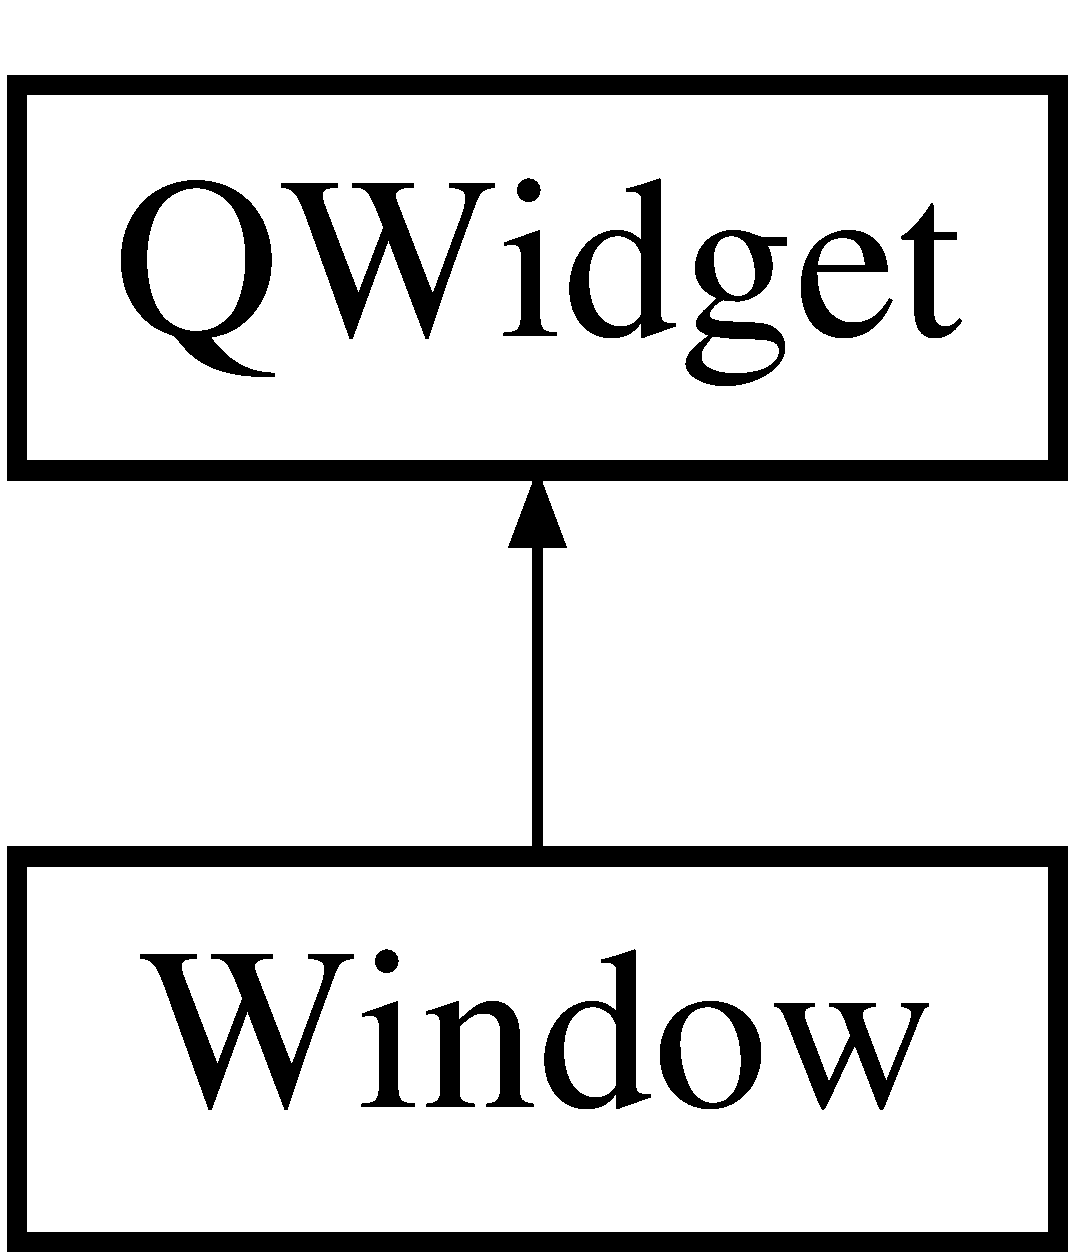
\includegraphics[height=2.000000cm]{classWindow}
\end{center}
\end{figure}
\subsection*{Public Slots}
\begin{DoxyCompactItemize}
\item 
\hypertarget{classWindow_a2733bcfa9a07113324b66e01a89a1fb8}{void {\bfseries connect} ()}\label{classWindow_a2733bcfa9a07113324b66e01a89a1fb8}

\item 
\hypertarget{classWindow_a96a44a2584b9848d058aadff91ce4d20}{void {\bfseries disconnect} ()}\label{classWindow_a96a44a2584b9848d058aadff91ce4d20}

\item 
\hypertarget{classWindow_a59515fc5a56e86d5a46d771595daac55}{void {\bfseries update} ()}\label{classWindow_a59515fc5a56e86d5a46d771595daac55}

\end{DoxyCompactItemize}
\subsection*{Public Member Functions}
\begin{DoxyCompactItemize}
\item 
\hypertarget{classWindow_aad5118913017eb418cab8b4c216f57aa}{void {\bfseries init\-Window} ()}\label{classWindow_aad5118913017eb418cab8b4c216f57aa}

\item 
\hypertarget{classWindow_af2ff981e828f1aa24957e8080fed33a4}{void {\bfseries init\-Widgets} ()}\label{classWindow_af2ff981e828f1aa24957e8080fed33a4}

\end{DoxyCompactItemize}


\subsection{Detailed Description}
Main window of the G\-U\-I. 

This class allows to instanciate, organize and update the qt and qwt widgets used for the display. \par
We can also connect or disconnect from the drone and get the drone's position in real time thanks to an udp\-Socket attribute. 

The documentation for this class was generated from the following files\-:\begin{DoxyCompactItemize}
\item 
/home/mathieu/drone-\/project/pc-\/linux/src/Window.\-h\item 
/home/mathieu/drone-\/project/pc-\/linux/src/Window.\-cpp\end{DoxyCompactItemize}

%--- End generated contents ---

% Index
\newpage
\phantomsection
\addcontentsline{toc}{chapter}{Index}
\printindex

\end{document}
